%--------------------
% Packages
% -------------------
\documentclass[11pt,a4paper]{article}
\usepackage[utf8x]{inputenc}
\usepackage[english]{babel}
\usepackage[T1]{fontenc}
%\usepackage{gentium}
% \usepackage{mathptmx} % Use Times Font


\usepackage[pdftex]{graphicx} % Required for including pictures
\usepackage[swedish]{babel} % Swedish translations
\usepackage[pdftex,linkcolor=black,pdfborder={0 0 0}]{hyperref} % Format links for pdf
\usepackage{calc} % To reset the counter in the document after title page
\usepackage{enumitem} % Includes lists
\usepackage{hyperref} % url


\frenchspacing % No double spacing between sentences
\linespread{1.2} % Set linespace
\usepackage[a4paper, lmargin=0.1666\paperwidth, rmargin=0.1666\paperwidth, tmargin=0.1111\paperheight, bmargin=0.1111\paperheight]{geometry} %margins
%\usepackage{parskip}

\usepackage[all]{nowidow} % Tries to remove widows
\usepackage[protrusion=true,expansion=true]{microtype} % Improves typography, load after fontpackage is selected

\usepackage{lipsum} % Used for inserting dummy 'Lorem ipsum' text into the template


\usepackage{float} % to fixate images

%-----------------------
% Set pdf information and add title, fill in the fields
%-----------------------
\hypersetup{ 	
pdfsubject = {02450 - Introduction to Machine Learning and Data mining},
pdftitle = {Project 1}
}

%-----------------------
% Begin document
%-----------------------
\begin{document} 



\title{Introduction to Machine learning and Data mining - Project 1} % Title


\begin{figure}
    \centering
    
\includegraphics[width=0.1\textwidth]{res/dtu_logo.png}
\end{figure}

% \author{Ivan Antonino Arena - s233352 \\
%  Nathan Lacour - s232062 \\
%  Nicolò Francesco Resmini - s231858  }  % Authors
 
\date{\today}

\maketitle
\begin{table}
\centering
\begin{tabular}{|l|c|c|c|c|c|c|}
 \hline
 \textbf{Student} & \textbf{ID} & \textbf{§1} & \textbf{§2} & \textbf{§3} & \textbf{§4} & \textbf{Exam quest.} \\
 \hline
 Ivan Antonino Arena & s233352 & 10\%  & 60\%  & 40\%  & 60\% & 33,33\%  \\
 \hline
 Nathan Lacour & s232062 & 40\%  & 10\%  & 0\%  & 10\%  & 33,33\%  \\
 \hline
 Nicolò Francesco Resmini & s231858 & 50\% & 30\%  & 60\%  & 30\%  & 33,33\% \\
 \hline
\end{tabular}
\end{table}


\pagebreak
\tableofcontents

\pagebreak

\section{Dataset Description}

% \subsection{Introduction}
The dataset that we selected contains data about the use of automatic rental bikes; all the processes are automatic as bikes are all connected to the net, thus it is possible to obtain a lot of interesting information about traffic (the duration of travel, starting position of the bike and its final location). Then, the rental bikes might be used as sensors that would give us knowledge about mobility in the city.

Bike-sharing rental process is highly influenced by parameters like the weather conditions or the time of the year, and in our data set we know the number of bikes that have been rented as well as when they were rented and additional information about the weather.

The data set is available on the UC Irvine website at the following address: \url{https://archive.ics.uci.edu/dataset/275/bike+sharing+dataset}.

The provided folder contained two versions of the dataset: \textit{day.csv} and \textit{hour.csv}, which only differ from one another for the $hr$ column, representing the hour of the day, not available in \textit{day.csv}. In light of this, we chose to use \textit{hour.csv} since it provides more accurate information, as the number of bikes rented in a day might heavily depend on the hour. \\


\subsection{Previous analysis of the data}
The Bike Sharing Dataset has been cited in more than ten scientific papers (referred in the same webpage from which we downloaded the dataset), which clearly demonstrates its breadth and its utility in supporting high-quality research. Therefore, we picked two of those papers and read them carefully to understand how this dataset had been used by the authors in their works.

The first one is “\textit{Recurrent Neural Networks for Time Series Forecasting}” by G'abor Petneh'azi (2019), which presents a recurrent neural network-based time series forecasting framework covering features engineering, features importance, points and intervals predictions, and forecast evaluations. Briefly, RNNs are essentially neural networks with memory, so they can remember things from the past, which is obviously useful for predicting time-dependent targets. Moreover, the author disregards the available weather information, and uses time-determined features only; he encodes the cyclical features (season of year, month of year, week of year, day of week and hour of day) through the use the sine and cosine transformations and he creates some binary variables, which are used to indicate if the time is afternoon, working hour, holiday, working day. 
Finally, to perform the value forecasts (regression) he also calculates variables importance by applying two different accuracy metrics (called R2 and MDA). In the end, the author states that he has reached good results, although he admits that even this 2-year hourly bike sharing dataset is way too small to exploit the capabilities of a neural network.

The second Paper examined is “\textit{D-vine quantile regression with discrete variables}” by Niklas Schallhorn, Daniel Kraus, Thomas Nagler, Claudia Czado (2017), which introduces new quantile regression (i.e. the prediction of statistical measures called conditional quantiles) approaches to handle the presence of mixed discrete-continuous data in a dataset, like ours. In fact, for each day we have continuous covariates temperature (Celsius), wind speed (mph) and humidity (relative in \%); additionally, there is the discrete variable weather situation giving information about the overall weather with values 1 (clear to partly cloudy), 2 (misty and cloudy) and 3 (rain, snow, thunderstorm). Eventually, by applying these new methods, prediction results show some dependencies between the features like “\textit{for temperatures higher than 32 degrees Celsius, each additional degree causes a decline in bike rentals}” or “\textit{bike rentals increase up to a relative humidity of around 60\% and decrease afterwards}”. 

Both these papers were really helpful to gain a deeper insight into the dataset, by making us look at the dataset from a different perspective and draw inspiration for some possible implementations of our project. \\

\subsection{Techniques}
With this data, we might be able to train a model to estimate how many people would rent a bike on a certain day with given weathers conditions. This could be useful for the people in charge of managing the city accommodations or planning events.

\begin{itemize}

\item \textbf{Regression:} by looking at the data it appears to us that the output that fits the regression task the best would be the number of users (either casual, registered or total), since, for example, it might be useful to get information about traffic congestion in the city. Moreover, we can also use almost all the other attributes as predictors ($weekday$, $workingday$, $holiday$, $mnth$, $hr$, $weathersit$, $temp$, $atemp$, $hum$, $windspeed$). 

% TODO: change weathersit with atemp??
\item \textbf{Classification:} while it might not be the primary scope of our problem of interest, the most obvious choice at first glance would be to try to perform classification on the $weathersit$ attribute, for instance, using as features the attributes $temp$, $atemp$, $hum$, $windspeed$ and the time of the year ($mnth$ or $season$). 

 
\end{itemize}

\subsection{Pre-processing}
In order to carry out these tasks, after carefully analyzing our dataset, we decided to perform some pre-processing steps, which are both helpful to perform more accurate data-visualization and fundamental for the application of the techniques in the second project of this course.\\
Here are the solutions we opted for:

\begin{itemize}
    \item removing the useless attribute $instant$, which provides a unique integer identifier for every observation of the dataset in sequential order;
    \item removing the attribute $yr$ (year), because it's a binary variable (0: 2011, 1:2012) and since it only represent two consecutive years we think it's negligible; 
    \item removing the attribute $dteday$ (date) because it's redundant, since we already have the date represented through other attributes ($weekday$, $mnth$, $yr$, $season$, $holilday$, $workingday$);
    \item applying the Square-Root transformation to the attribute $cnt$, which is the count of total rental bikes including both casual and registered, to transform it in a continuous variable (by using the \textit{sqrt} function) to perform regression on it. As it is also explained in the paper "\textit{Anchor regression: heterogeneous data meet causality}" (Rothenhausler et al., 2020), this is a common procedure and fits reasonably well the assumptions to make it valid;
    \item removing the attributes $casual$ and $registered$, which became deprecated after the square-root transformation of $cnt$, since $cnt$ was equal to the sum of the two attributes.
\end{itemize}


    
   

    
\section{Attributes of the data}

\subsection{Attributes list}

\begin{center}
\begin{tabular}{|l|c|c|p{7cm}|}
\hline
\textbf{Attribute} & \textbf{Type} & \textbf{Measurement} & \textbf{Description} \\
\hline
instant & Discrete & Interval & Number of the observation. \\
\hline
dteday & Discrete & Interval & Date in YYYY-MM-DD format. \\
\hline
season & Discrete & Nominal & Encoded seasons (1: Winter, 2: Spring, 3: Summer, 4: Fall). \\
\hline
yr & Discrete & Nominal & Year (0: 2011, 1: 2012). \\
\hline
mnth & Discrete & Nominal & Number of the month in year. \\
\hline
hr & Discrete & Interval & Hour in day (24 hours). \\
\hline
holiday & Discrete & Nominal & 1 if day is holiday, else 0. \\
\hline
weekday & Discrete & Nominal & Number of day in week. \\
\hline
workingday & Discrete & Nominal & 1 if day is working day, else 0. \\
\hline
weathersit & Discrete & Ordinal & Encoded weather situation (1: Clear, Few clouds, Partly cloudy, Partly cloudy, 2: Mist + Cloudy, Mist + Broken clouds, Mist + Few clouds, Mist, 3: Light Snow, Light Rain + Thunderstorm + Scattered clouds, Light Rain + Scattered clouds, 4: Heavy Rain + Ice Pallets + Thunderstorm + Mist, Snow + Fog). \\
\hline
temp & Continuous & Ratio & Normalized temperature in Celsius. The values are derived via (t-t\_min)/(t\_max-t\_min), t\_min=-8, t\_max=+39 (only in hourly scale). \\
\hline
atemp & Continuous & Ratio & Normalized feeling temperature in Celsius. The values are derived via (t-t\_min)/(t\_max-t\_min), t\_min=-16, t\_max=+50 (only in hourly scale). \\
\hline
hum & Continuous & Ratio & Normalized humidity. The values are divided to 100 (max). \\
\hline
windspeed & Continuous & Ratio & Normalized wind speed. The values are divided to 67 (max). \\
\hline
casual & Discrete & Ratio & Count of casual users. \\
\hline
registered & Discrete & Ratio & Count of registered users. \\
\hline
cnt & Discrete & Ratio & Count of total rental bikes including both casual and registered. \\
\hline
\end{tabular}
\end{center}




\subsection{Data issues}

After carefully analyzing the dataset, we can confidently say that there are no missing values or corrupted data, therefore no statistical techniques to replace eventual missing values with reasonable approximations should be performed. As a confirmation, the same conclusion has been reached in the paper “\textit{VINE: Visualizing Statistical Interactions in Black Box Models}” (Matthew Britton, 2019).

\subsection{Summary statistics}


\begin{figure}[H]
    \centering
    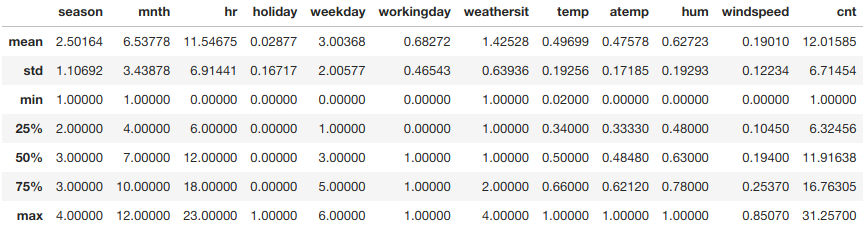
\includegraphics[width=\textwidth]{res/statistics_summary.png}
    \caption{Summary statistics for the dataset.}
    \label{fig:summary}
\end{figure}



\section{Data visualization and PCA}

\subsection{Outliers}


By standardizing all data and plotting them to a box plot, there appear some possible outliers: $holiday$, $weathersit$, $hum$, $windspeed$.
We can soon exclude any issue with the $holiday$ attribute because it's binary, therefore explaining the suspicious result in the plot. After a further examination of the attributes, we decided to keep the other three attributes as they are, despite the evident discrepancies in the values, because they represent physical phenomena and we don't know how they have been measured, thus we assume that the values are all truthful. \\
In addition, we have plotted histograms regarding the outliers distributions for these attributes, which can be found in Appendix \ref{appendix:plots}.

\begin{figure}[H]
    \centering
    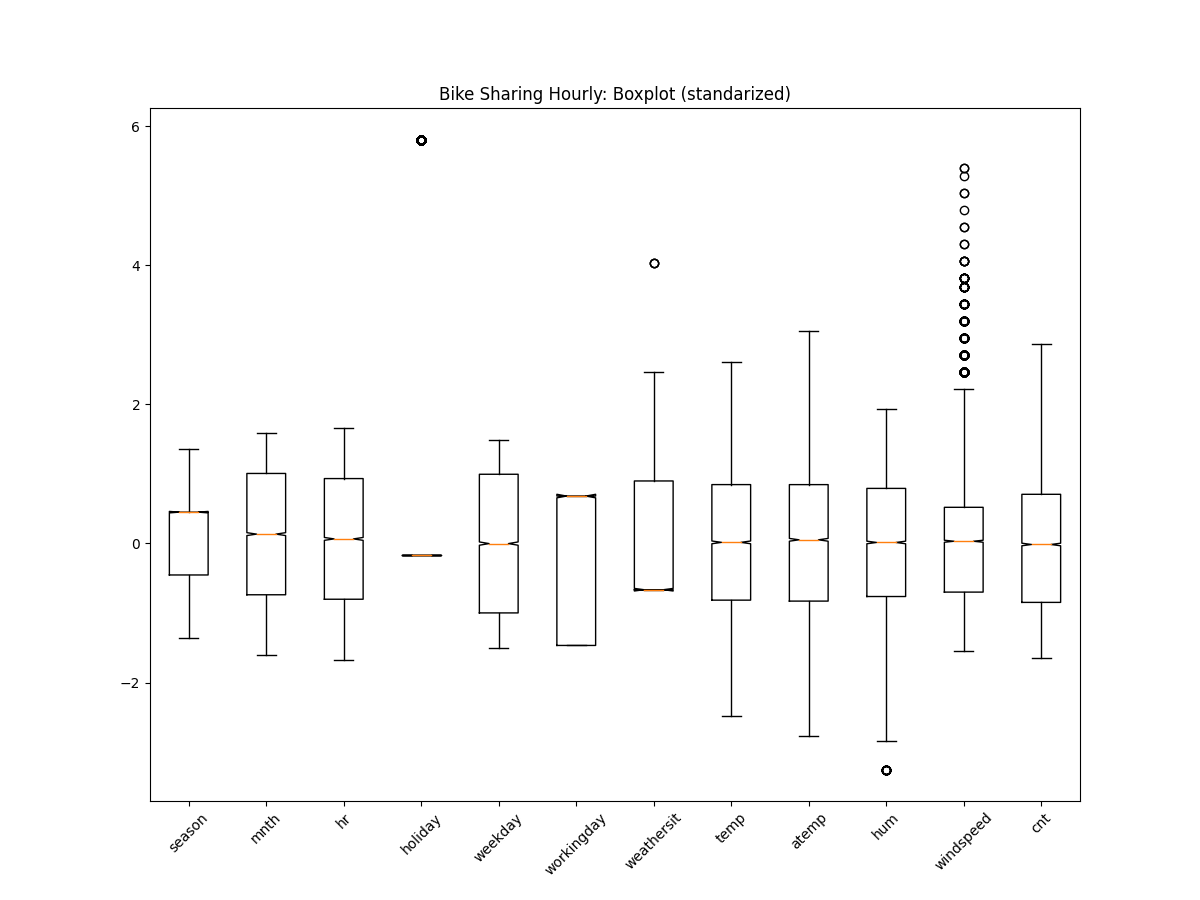
\includegraphics[width=1.0\linewidth]{res/plots/boxplot_standardized.png}
    \caption{Standardized boxplot of the dataset.}
    \label{fig:boxplot}
\end{figure}


\subsection{Normal distribution}

As a consequence of being visualized in a histogram comprised of 1000 data samples, with a theoretical mean of 0 and a theoretical standard deviation of 2, the dataset reasonably showcases a bell-shaped, symmetrical distribution, resembling the characteristic shape of a normal distribution curve. This empirical observation suggests that the data adheres enough to the theoretical model of a normal distribution.

\begin{figure}[H]
    \centering
    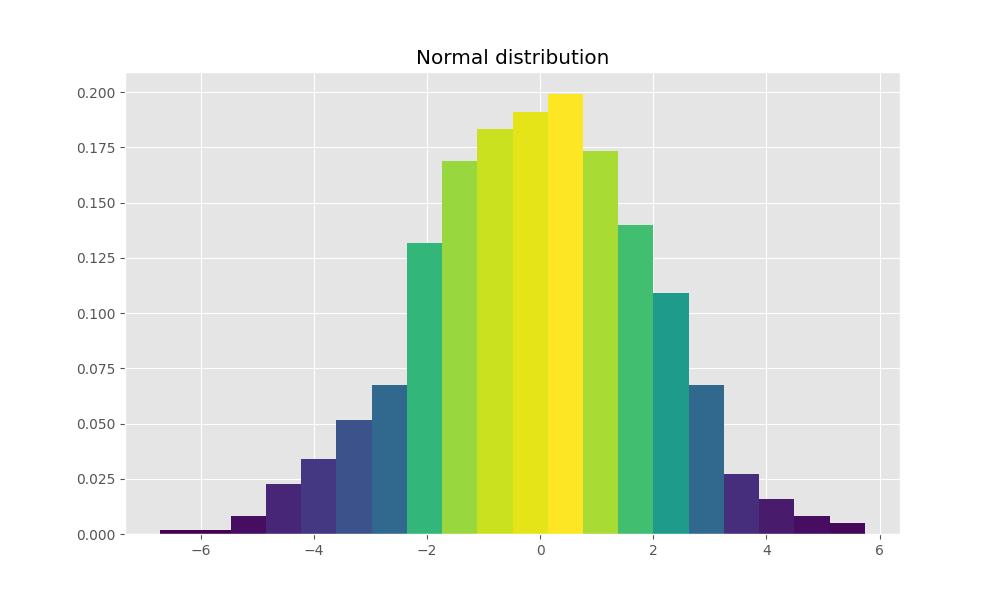
\includegraphics[width=0.6\linewidth]{res/plots/normal_distribution.png}
    \caption{Histogram of the data for normal distribution.}
    \label{fig:normal}
\end{figure}

\subsection{Correlation}

We have generated a comprehensive correlation heat-map to explore the interrelationships among the attributes within our dataset. This graphical representation serves as a valuable tool, offering us a valuable perspective on how various variables are associated.

Upon close examination, it becomes evident that the most pronounced correlations are observed between $cnt$ and $hr$, $temp$, $atemp$, and $hum$. These strong associations imply that $cnt$ could be a highly suitable choice as the target variable in any subsequent regression analysis, given its discernible connection with these predictor variables. 

We have also noticed that, among the candidate attributes for classification, both $temp$ and $atemp$ (which represent, respectively, the actual and perceived temperature) exhibit noteworthy correlations with attributes such as $season$, $mnth$, $hr$ and $cnt$: this observation suggests that either one of these two attributes could be promising candidates for the output variable in a classification task.

However, it's important to note that $temp$ and $atemp$ are normalized continuous variables, therefore there will be the need to transform one of them into a discrete variable to make it suitable for the classification tasks.


\begin{figure}[H]
    \centering
    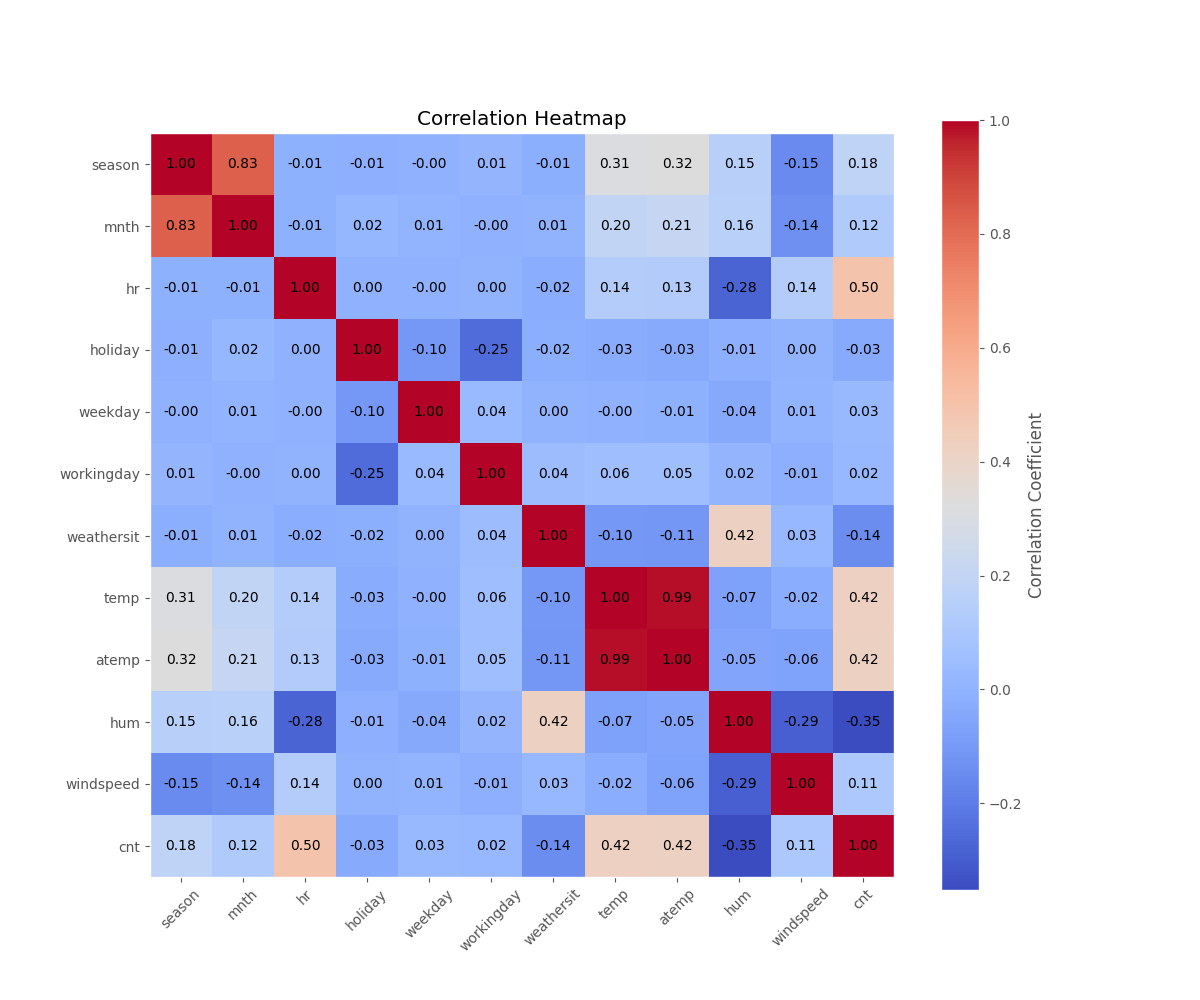
\includegraphics[width=0.9\linewidth]{res/plots/correlation_heatmap.png}
    \caption{Heat-map of the correlation between attributes.}
    \label{fig:correlation_heatmap}
\end{figure}

Furthermore, we took a closer look to attributes with the highest correlation with $cnt$, plotting them to scatter plots to have a clearer overview of the trends. These plots can be found at the end of this document, in Appendix \ref{appendix:plots}.

\subsection{PCA}

To gain deeper insights into the underlying structure of our dataset, we have employed Principal Component Analysis (PCA), which is a powerful feature extraction technique that allows us to visualize and explore the patterns and relationships within high-dimensional data.
Before performing it, we standardized the data by adjusting for differing scales among attributes before plotting the various PCA analysis.

First of all, we created a plot that illustrates the amount of variation explained as we progressively include additional PCA components. This visual representation provided us with valuable information about the dimensionality reduction and the retained information when selecting different numbers of PCA components.

\begin{figure}[H]
    \centering
    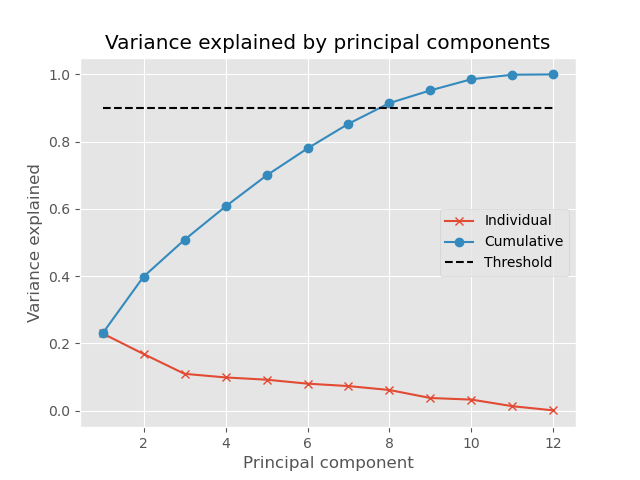
\includegraphics[width=0.8\linewidth]{res/plots/variance_explained.png}
    \caption{Variation explained as a function of the number of PCA
components included.}
    \label{fig:/variance_explained}
\end{figure}

As we can see from the plot above, to reach the threshold of 90\% cumulated variance we need to include at least the first 8 principal components.

Moreover, in pursuit of a deeper understanding of our dataset's structure, we needed to visualize the principal directions associated with the considered PCA components. The plot below enabled us to gain insights into the primary axes of variation captured by PCA, providing valuable information about the dominant patterns and relationships within our data.

\begin{figure}[H]
    \centering
    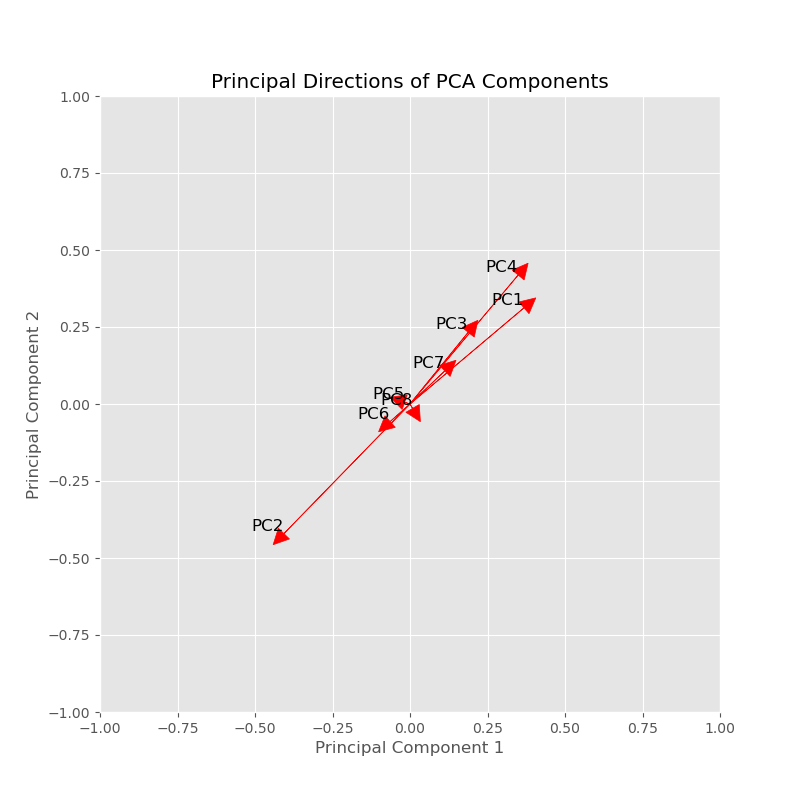
\includegraphics[width=0.7\linewidth]{res/plots/pca_components.png}
    \caption{Principal directions of the considered PCA components.}
    \label{fig:/pca_components}
\end{figure}

In the end, we have plotted the data projected onto the two most significant principal components, which allows us to explore the dataset in a reduced-dimensional space, shedding light on how the data distributes and varies along these principal axes.

\begin{figure}[H]
    \centering
    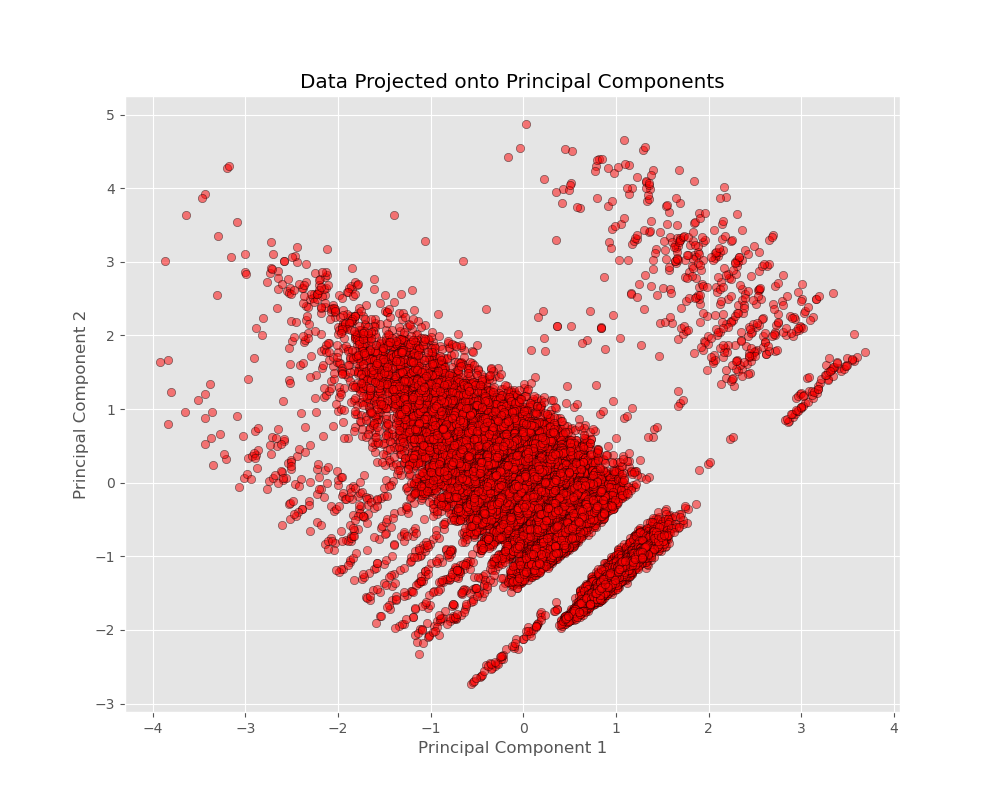
\includegraphics[width=0.7\linewidth]{res/plots/pca_projected.png}
    \caption{Data projected onto the first two principal components.}
    \label{fig:/pca_projected}
\end{figure}


\section{Conclusion}

Overall, the Bike Sharing Dataset (hourly) appears to be suitable for supervised learning. The absence of outliers or noise make it a high quality dataset, furthermore, most of the attributes come already scaled and normalized, allowing the data engineering operations to be minimal on our part, consisting only in ignoring some of the attributes because of redundancy ($dteday$, $casual$, $registered$) or irrelevance($instant$, $yr$) and applying the square root to the $cnt$ attribute to make it continous, therefore suitable as a target variable for linear regression.
Given our visualizations, the dataset also appears to be normally distributed and featuring relevant levels of correlation between some of the attributes allowing it to be used optimistically for regression and classification tasks.  For the regression task, for instance, we could use the $cnt$ attribute as a target variable, as it appears to be highly correlated with $hr$, $temp$, $atemp$ and $hum$. As per the classification task, contrary to our belief stated in §1, the attributes $temp$ or $atemp$ seem to be more promising attributes than $wheatersit$.
Finally, the only potential drawback to the dataset is that, despite the high number of observations, the data has been collected over the span of two years, thus potentially penalizing an eventual model in seeing long-term trends or cyclical patterns.

\pagebreak
\appendix
\label{appendix:ex}
\section{Exercises solutions}

\subsection{Question 1}

\paragraph*{Answer:} C.
\paragraph*{Solution:} 
$x_1$ is interval because it describes 30-minute intervals, therefore the distance between one value from the consecutive one is fixed and it has an order since $x_1 = 1$ corresponds to the interval 7:00-7:30, which is sooner in time than the following intervals; $x_6$ is ratio because it's a number and it has a true zero ($x_6 = 0$ means that there are no broken traffic lights); $x_7$ is ratio for the same reason ($x_7 = 0$ means that there are no run over accidents); $y$ is ordinal since it takes values that can be ranked, in this case, from no congestion to a high level of congestion.

\subsection{Question 2}

\paragraph*{Answer:} A.
\paragraph*{Solution:} the $\infty$-norm distance between $x_{14}$ and $x_{18}$ is 7.0 because it's indeed the maximum of the absolute value of the differences between the coordinates of the two vectors: max\{|26-19|, |2-0|, 0\} = 7.0


\subsection{Question 3}

\paragraph*{Answer:} A.
\paragraph*{Solution:} the variation explained by each principal component is given by $\frac{\sigma_i^2}{\sum_{i'} \sigma_{i'}^2}$, where $\sigma_i$ is the singular value related to the principal component $i$. In this case: $\frac{13.9^2+12.47^2+11.48^2+10.03^2}{13.9^2+12.47^2+11.48^2+10.03^2+9.45^2} = 0,867 > 0,8$

\subsection{Question 4}

\paragraph*{Answer:} D
\paragraph*{Solution:}  The columns of V represents the directions of each PCA. Given that fact, an observation would have a positive value of the projection onto a
principal component if each of its components have the same signs as the components of the eigenvector related to the principal component in question. Moreover, since we substract the mean value of each caracteristic , a low value mean that the projection will have a negative component for that caracteristic, in the same way, a high value will give a positive component. If we follow that logic the only fitted answer is D.

\subsection{Question 5}

\paragraph*{Answer:} A.
\paragraph*{Solution:} The formula for Jaccard similarity is the following: $J(x,y) = \frac{f_{11}}{K-f_{00}}$, where $K = M = 20000$, $f_{11} = 2$ because it's the number of words present in both $s_1$ and $s_2$ ("the", "words"), $f_{00} = 20000 - 13 = 19987$ because it's the number of words that are missing in both $s_1$ and $s_2$, therefore all the words except the ones that are present counted only once ("the", "bag", "of", "words", "representation", "becomes", "less", "parsimoneous", "if", "we", "do", "not", "stem"). Thus, $J(x,y) = \frac{f_{11}}{K-f_{00}} = \frac{2}{20000 - 19987}= \frac{2}{13} = 0.153846$. 

\subsection{Question 6}

\paragraph*{Answer:} B
\paragraph*{Solution:} If we consider that $P(B|C) = P(AB|C) + P(\overline{A}B|C)$ and given the binary nature of $x_2$ and $x_7$ we get that $P(x_2 = 0 | y = 2) = P(x_2 = 0, x_7 = 0 | y = 2) + P(x_2 = 0, x_7 = 1 | y = 2) $ considering that $A = "x_7 = 0"$, $\overline{A} = "x_7 = 1"$, $B = "x_2 = 0"$ and $C = "y = 2"$.

\section{Additional Plots}
\label{appendix:plots}
\subsection{Distribution of outliers}

\begin{figure}[H]
    \centering
    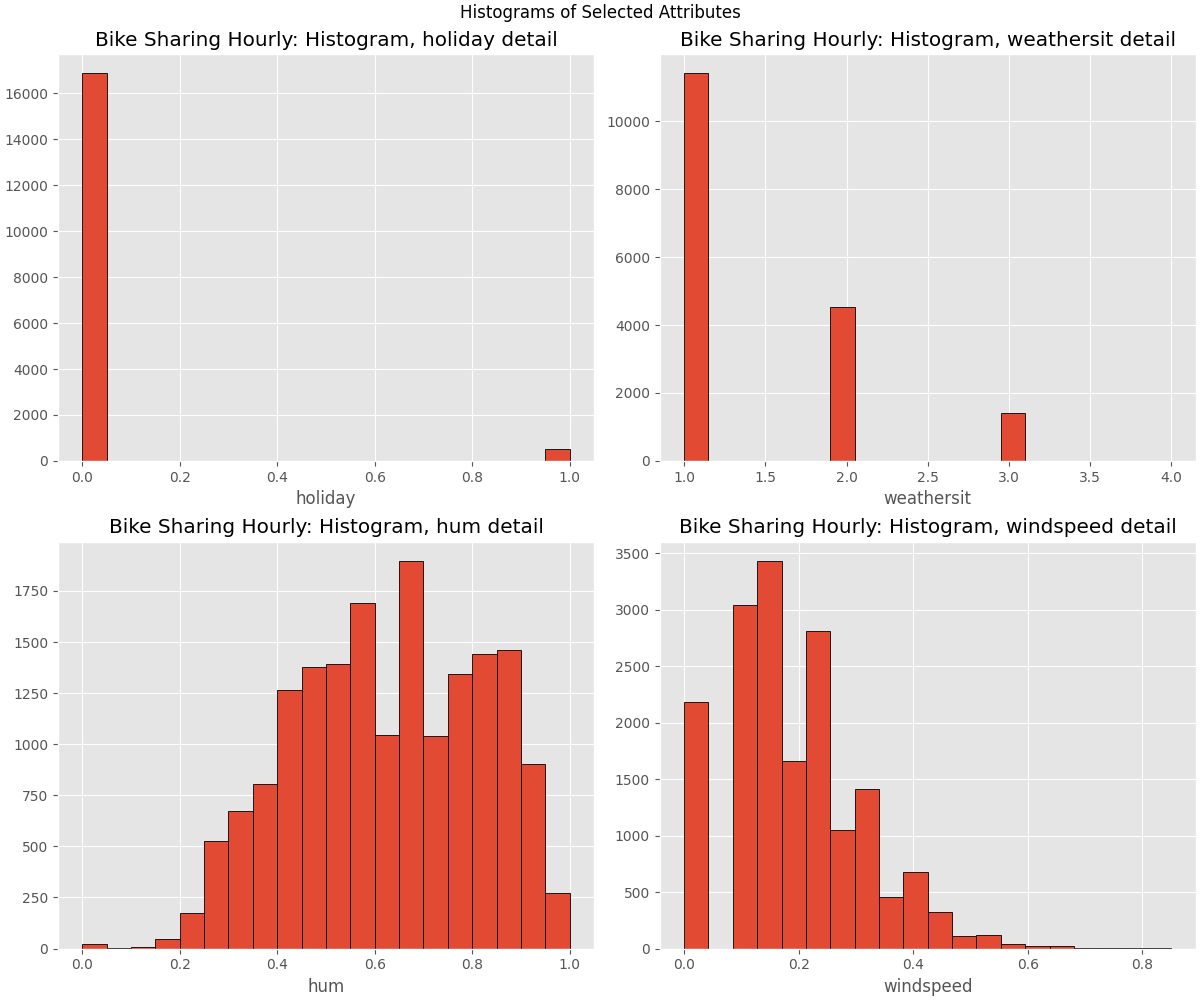
\includegraphics[width=1\linewidth]{res/plots/hist_multiple_attributes.png}
    \caption{Histograms detail of \textit{holiday}, \textit{weathersit}, \textit{hum} and \textit{windspeed} attributes.}
    \label{fig:hist_detail}
\end{figure}

\subsection{Correlation between $cnt$ and some attributes}

\begin{figure}[H]
    \centering
    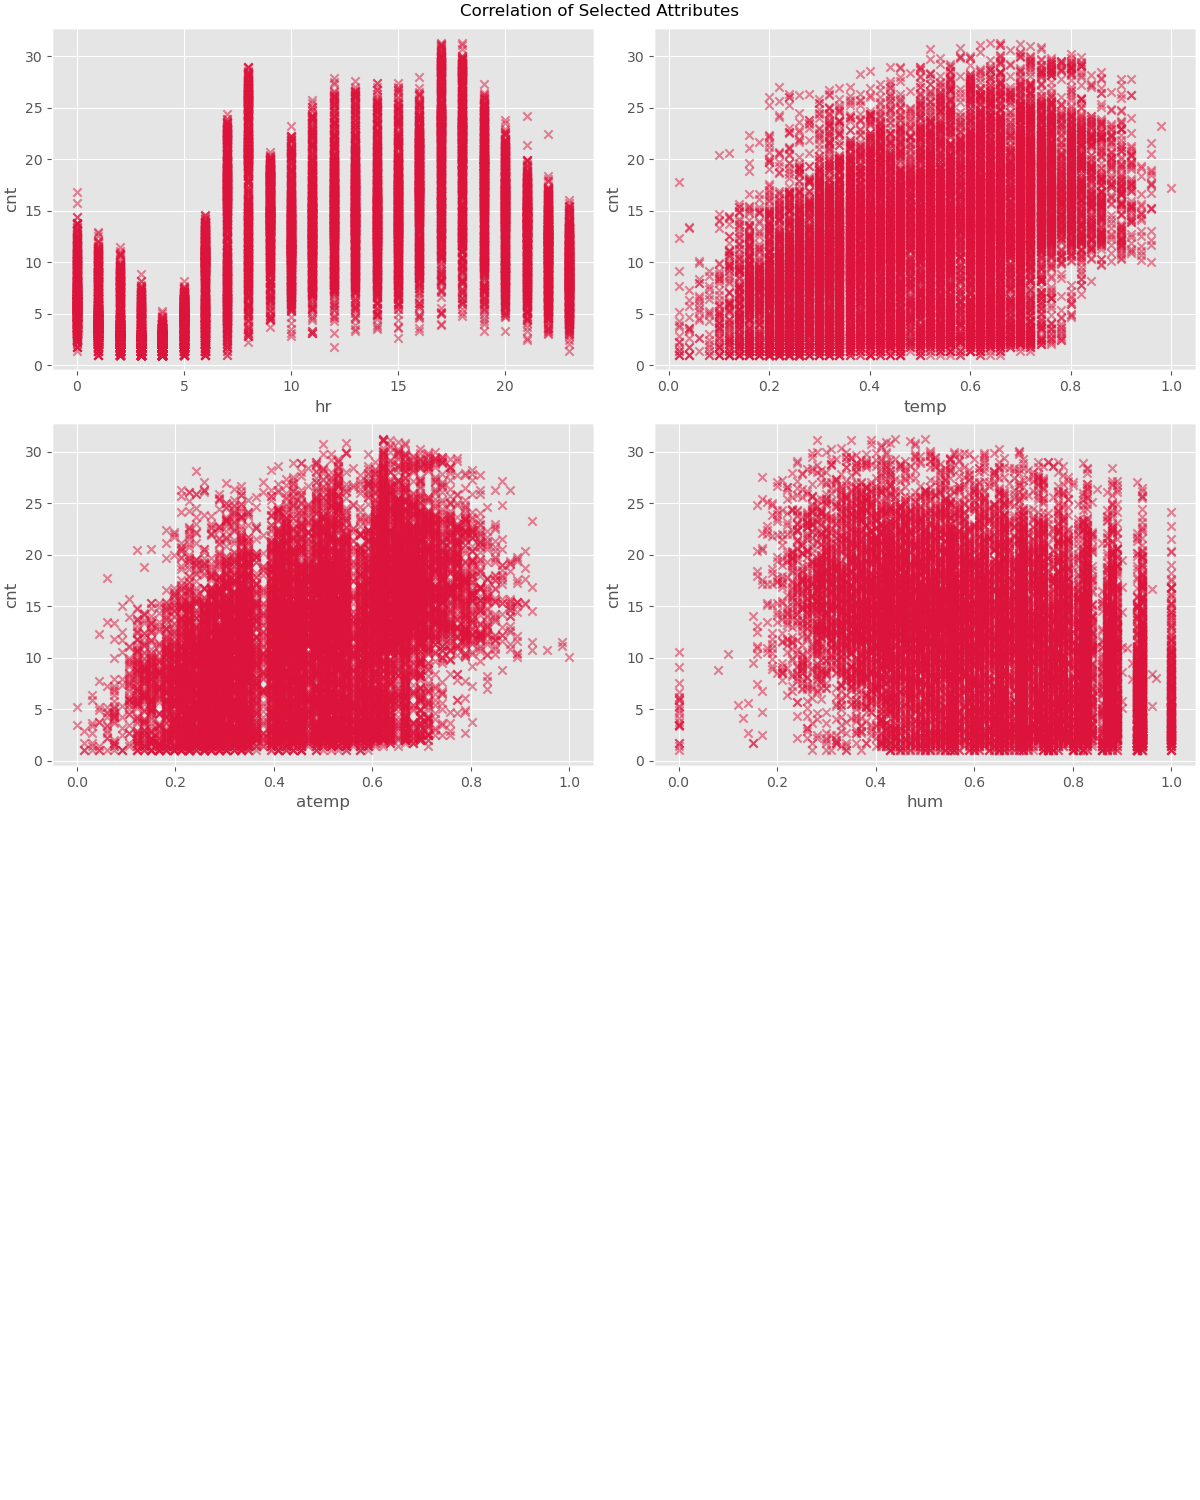
\includegraphics[width=\linewidth]{res/plots/correlation.png}
    \caption{Scatter plots of $cnt$ against $hr$, $temp$, $atemp$ and $hum$.}
    \label{fig:correlation}
\end{figure}

\end{document}

